\documentclass[paper=a4, fontsize=11pt]{scrartcl} 

\usepackage[T1]{fontenc} 
\usepackage[english]{babel}
\usepackage{amsmath,amsfonts,amsthm}

\usepackage{lipsum}

\usepackage{graphicx}
\usepackage{float}
  \floatplacement{figure}{H}
  \floatplacement{table}{H}
  
\usepackage{sectsty} 
\allsectionsfont{\centering \normalfont\scshape} 

\usepackage{fancyhdr} % Custom headers and footers
\pagestyle{fancyplain} % Makes all pages in the document conform to the custom headers and footers
\fancyhead{} % No page header - if you want one, create it in the same way as the footers below
\fancyfoot[L]{} % Empty left footer
\fancyfoot[C]{} % Empty center footer
\fancyfoot[R]{\thepage} % Page numbering for right footer
\renewcommand{\headrulewidth}{0pt} % Remove header underlines
\renewcommand{\footrulewidth}{0pt} % Remove footer underlines
\setlength{\headheight}{13.6pt} % Customize the height of the header

\usepackage[labelformat=empty]{caption}
\usepackage{color}
\usepackage{listings}
\lstset{ %
language=bash,                % choose the language of the code
basicstyle=\footnotesize,       % the size of the fonts that are used for the code
numbers=left,                   % where to put the line-numbers
numberstyle=\footnotesize,      % the size of the fonts that are used for the line-numbers
stepnumber=1,                   % the step between two line-numbers. If it is 1 each line will be numbered
numbersep=5pt,                  % how far the line-numbers are from the code
backgroundcolor=\color{white},  % choose the background color. You must add \usepackage{color}
showspaces=false,               % show spaces adding particular underscores
showstringspaces=false,         % underline spaces within strings
showtabs=false,                 % show tabs within strings adding particular underscores
frame=single,           % adds a frame around the code
tabsize=2,          % sets default tabsize to 2 spaces
captionpos=b,           % sets the caption-position to bottom
breaklines=true,        % sets automatic line breaking
breakatwhitespace=false,    % sets if automatic breaks should only happen at whitespace
escapeinside={\%*}{*)}          % if you want to add a comment within your code
}
\usepackage{hyperref}


\numberwithin{equation}{section} % Number equations within sections (i.e. 1.1, 1.2, 2.1, 2.2 instead of 1, 2, 3, 4)
\numberwithin{figure}{section} % Number figures within sections (i.e. 1.1, 1.2, 2.1, 2.2 instead of 1, 2, 3, 4)
\numberwithin{table}{section} % Number tables within sections (i.e. 1.1, 1.2, 2.1, 2.2 instead of 1, 2, 3, 4)

\setlength\parindent{0pt} % Removes all indentation from paragraphs - comment this line for an assignment with lots of text

%----------------------------------------------------------------------------------------
%	TITLE SECTION
%----------------------------------------------------------------------------------------

\newcommand{\horrule}[1]{\rule{\linewidth}{#1}} % Create horizontal rule command with 1 argument of height

\title{	
\normalfont \normalsize 
\textsc{Computational Science} \\ [25pt] % Your university, school and/or department name(s)
\horrule{0.5pt} \\[0.2cm] % Thin top horizontal rule
\small Homework - Introduction to Frontiers of Computational Science\\ % The assignment title
%\horrule{2pt} \\[0.5cm] % Thick bottom horizontal rule
}

\author{\small{Ridlo W. Wibowo || 1215011069}} % Your name

\date{\small October 28, 2013} % Today's date or a custom date


\begin{document}
\maketitle % Print the title

\textbf{Problem 1.}\\
Conservation or continuity in Maxwell's equation can be derived from Ampere's law and Gauss' law. Suppose we write out a vector identity that is always true, which states that the divergence of the curl of any vector field is always zero:
\begin{equation*}
\nabla \cdot ( \nabla \times \textbf{H} ) = 0
\end{equation*}
If we apply the divergence to Ampere's Law, we obtain:
\begin{eqnarray*}
\nabla \cdot \left( \frac{\partial \textbf{D}}{\partial t} + \textbf{J} \right) &=& \nabla \cdot ( \nabla \times \textbf{H} ) = 0\\
\frac{\partial (\nabla \cdot \textbf{D})}{\partial t} + \nabla \cdot \textbf{J} &=& 0
\end{eqnarray*}
and from the Gauss' law $(\nabla \cdot \textbf{D} = \rho)$:
\begin{eqnarray*}
\frac{\partial \rho}{\partial t} + \nabla \cdot \textbf{J} &=& 0\\
\nabla \cdot \textbf{J} &=& -\frac{\partial \rho}{\partial t} 
\end{eqnarray*}
The left side of the equation is the divergence of the Electric Current Density ($\textbf{J}$). This is a measure of whether current is flowing into a volume (i.e. the divergence of $\textbf{J}$ is positive if more current leaves the volume than enters). If charge is exiting, then the amount of charge within the volume must be decreasing. This is exactly what the right side is a measure of - how much electric charge is accumulating or leaving in a volume. Hence, the continuity equation is about continuity - if there is a net electric current is flowing out of a region, then the charge in that region must be decreasing. If there is more electric current flowing into a given volume than exiting, than the amount of electric charge must be increasing. (ref: \url{http://maxwells-equations.com/}).\\


\textbf{Problem 2.}\\
a. Solve this problem:
\begin{figure}
	\centering
	\includegraphics[width=0.3\textwidth]{2a.png}
\end{figure}
\begin{eqnarray*}
Q &=& k (T_1 - T_2)\\
\frac{d}{dt}(cT_1) &=& -Q\\
\frac{d}{dt}(cT_2) &=& +Q
\end{eqnarray*}
if the constants and initial value is given, find $T_1(t)$ and $T_2(t)$!\\


Answer:\\
Analitically:\\
\begin{eqnarray*}
\frac{d}{dt}(c(T_1 + T_2)) &=& 0\\
\frac{d}{dt}(c(T_1 - T_2)) &=& -2Q
\end{eqnarray*}
then,
\begin{eqnarray*}
\frac{d}{dt}(T_1 + T_2) &=& 0\\
\frac{d}{dt}(T_1 - T_2) &=& -2\mu(T_1 - T_2)
\end{eqnarray*}
with $\mu = k/c$,
\begin{eqnarray*}
(T_1 + T_2)_{(t)} &=& (T_1 + T_2)_{(0)}\\
(T_1 - T_2)_{(t)} &=& (T_1 - T_2)_{(0)} e^{-2 \mu t}
\end{eqnarray*}
using addition and substraction,
\begin{eqnarray*}
T_1 &=& \frac{T_1^{(0)}}{2} \left( 1 + e^{-2 \mu t} \right) + \frac{T_2^{(0)}}{2} \left( 1 - e^{-2 \mu t} \right)\\
T_2 &=& \frac{T_1^{(0)}}{2} \left( 1 - e^{-2 \mu t} \right) + \frac{T_2^{(0)}}{2} \left( 1 + e^{-2 \mu t} \right)
\end{eqnarray*}

\newpage
Numerically:\\
Using euler method directly from the problem, and using analitically solution above,
\begin{figure}
	\centering
	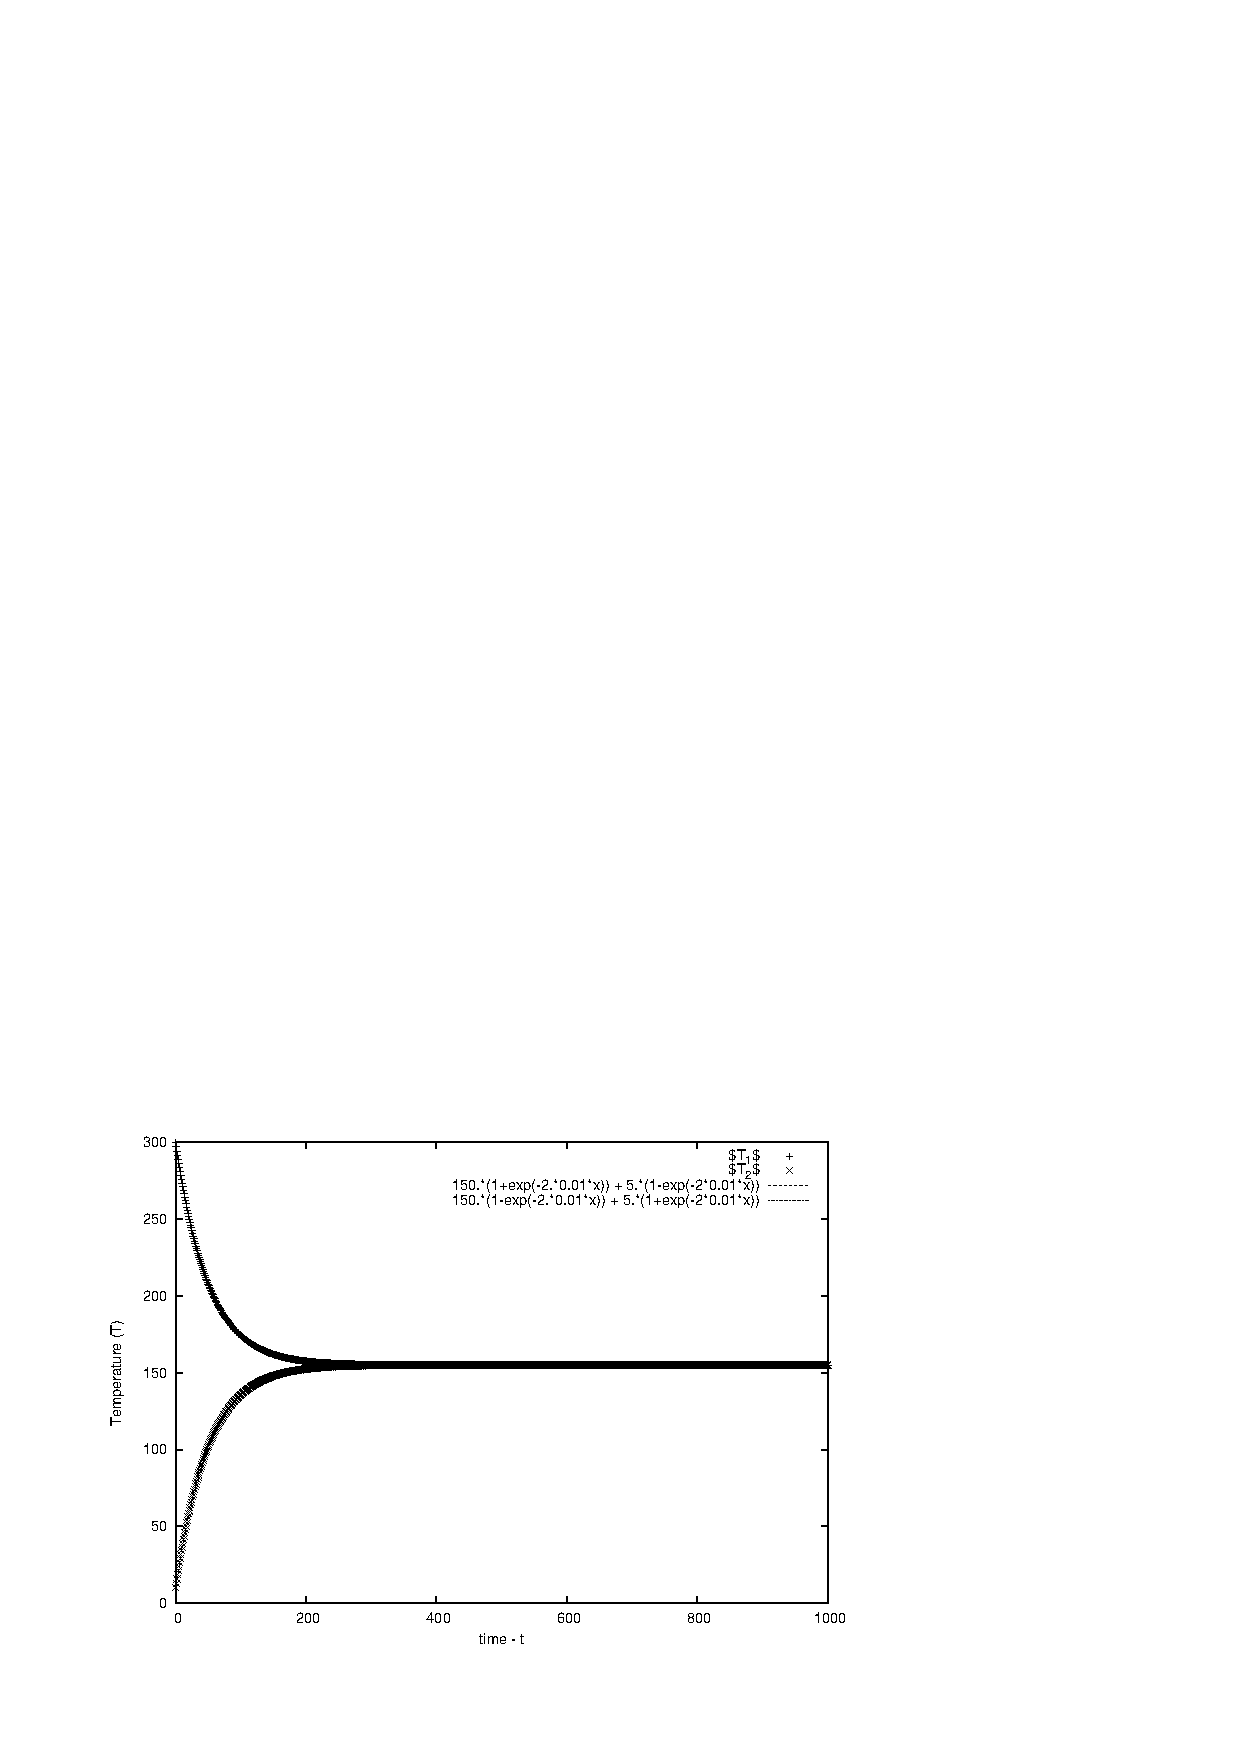
\includegraphics[width=0.7\textwidth]{num.png}
\end{figure}


b. Write the heat transfer equation for this problem:
\begin{figure}
	\centering
	\includegraphics[width=0.4\textwidth]{2b.png}
\end{figure}
Answer:
\begin{eqnarray*}
\frac{d}{dt}(T_1) &=& - \mu(T_1 - T_2)\\
\frac{d}{dt}(T_2) &=& \mu(T_1 - T_2) - \mu(T_2 - T_3)\\
\frac{d}{dt}(T_3) &=& \mu(T_2 - T_3)
\end{eqnarray*}

\end{document}